\section{System Overview}
In this section, we describe the application and system model behind \compiler\
to provide an understanding of where, and how, it may be deployed. We envision
DBToaster being packaged side-by-side with existing relational databases to
provide a complete data management solution that is both capable of processing
repeated or standing queries extremely efficiently through \compiler, and
processing unseen queries through existing query engines. 

\subsection{Application Model}
\compiler\ is capable of compiling a wide variety of SQL queries including those
containing selections, projections, joins, and group-by aggregates. \compiler\
takes a query workload as input, as well as the data definition statements of any
tables used in the queries to determine the contents of internal datastructures,
and produces a native binary for processing the query workload over inserts,
deletes and updates on the input tables. \compiler\ focuses on applications faced
with handling a large input volume, but does not rely on artificial restrictions
of these new inputs, unlike stream processing engines, which rely on semantic
constructs such as windows or punctuations that are tightly coupled with operator
semantics. Indeed, many stream applications, such as order book trading are
self-managing, in that the application logic and usage patterns ensures state
does not grow unbounded eliminating the need for windows. Otherwise, windows may
often be expressed as predicates. \compiler\ will compile such window semantics
just as with any other part of the query, and as we will see later, efficiently
implement windowing based on the data structures used to process the windowing
predicate.

At its core, \compiler\ performs delta processing, that is each insert, delete or
update of an input table is processed through the query and produces a new
result.
\compiler\ can support two types of result tuples, delta results or full
aggregate results. Internally \compiler\ computes one of these result types
depending on the type of aggregation function (for example full aggregation
results for a \texttt{max}), and maintains prior results to enable outputs of
either type. Furthermore, \compiler\ can produce both a standalone query engine
communicating both results and inputs through a socket interface, or an embedded
engine library that provides cursor-based access to full query results. This
cursor-based access is backed by internal datastructures created by \compiler\
for query processing, for example a hashtable of aggregate results keyed by
group-by columns.

  
\subsection{System Architecture}
\begin{figure}
\begin{center}
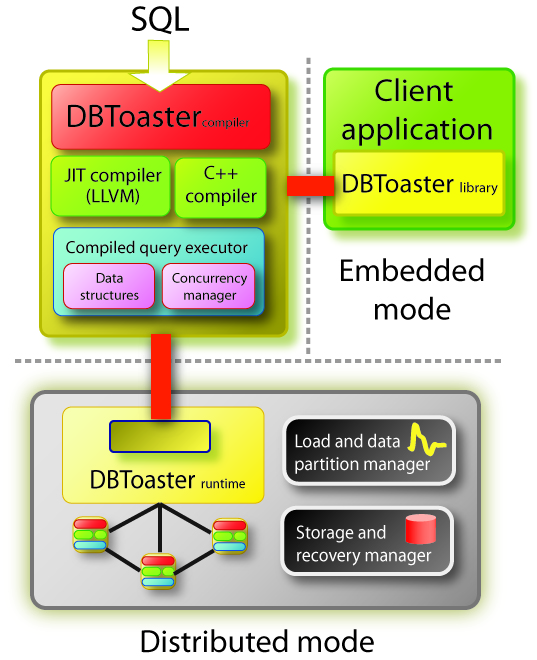
\includegraphics[scale=0.45]{figures/overview}
\end{center}
\caption{\compiler\ architecture diagram. \compiler\ can be used in a standalone
mode where it simply performs query processing, embedded mode where it can be
linked into another application and provide query result cursors, or finally as
a scalable distributed query processor.}
\label{fig:overview}
\end{figure}

While the main focus of this paper is on the compilation phase in \compiler, we
briefly describe the architecture of the system hosting our compiled
query executor, outlining our plans for addressing overarching systems issues
such as scalability, self-management, and reliability.

Despite increasing main-memory capacities presented as part of our motivation for
this work, for scalability, we foresee the need to extend beyond a single server
approach in two steps, to both a multi-core shared memory model, and a
distributed shared-nothing main-memory model. While the latter can be handled
gracefully by intelligent workload partitioning, the former requires
investigating concurrency control of our generated code as it processes inserts,
updates and deletes. Given our implementation of queries as a set of
highly-efficient straight-line functions, an event-based approach to concurrency
control appears to be a natural fit in this context, however we still face the
challenge of sharing data structures across generated functions. We plan to
investigate both lock-free and transactional memory techniques for these data
structures, as well as applying simplified program analysis techniques leveraging
properties of the relational algebra during compilation to extract parallelism
where possible.

Returning to the issue of scalability, any cluster-based deployment of \compiler\
will need to adapt to changing workload conditions and apply load management
techniques to efficiently use available resources and provide high performance
query processing. Given \compiler\ executes native binaries, rather than relying
on dynamic library interfaces such as \texttt{dlopen()} which suffer from binary
incompatibilities, our architecture uses a persistent lightweight distributed
runtime incorporating a just-in-time (JIT) compiler. By building on top of JIT
compilation, our architecture enables support for query migration and adaptation
at runtime at the logical, query, layer rather than in terms of binaries. We plan
on using the Low-Level Virtual Machine (LLVM) compilation framework as a JIT code
generator, ultimately having \compiler\ generate LLVM's intermediate
representation for subsequent native code generation. However, as an initial
step, we produce C++ code which can then be processed by the C++ frontend for
LLVM.

With the ability to migrate compiled queries, \compiler\ can begin to address
resource management challenges, solving a resource optimization problem based on
the tradeoff in achieving a balanced load allocation in the cluster, and
providing high throughput by localizing queries with the data they access. The
layout challenge in \compiler's context differs from traditional distributed data
placement problems in that we are using data structures rather than relations,
requiring consideration of distributed data structures (hashtables, trees, etc.)
and novel partitioning schemes for these data structures.
\comment{
Additionally query groupings have to be managed in order to exploit the
potential data structure sharing amongst multiple queries.
}
Other key system components include a storage and recovery manager responsible
for checkpointing and managing the handoff of checkpoints to backups to provide
fault tolerance in our purely main-memory context, as well as providing and
managing secondary storage primarily for the purpose of data loading and shipping
to ensure maximal availability of main-memory for query processing purposes
rather than distributed system maintenance.

\comment{
\begin{itemize}
  \item \compiler\ compiles SQL down to C code, and this compiler is the main
  focus of this paper.

  \item For scalability and availability reasons, we foresee implementing a
  distributed lightweight runtime consisting of several additional
  components. This runtime will behave much more like a JIT compiler for runtime
  adaptivity, maintaining persistent versions of our compiler's metadata, and
  dynamically generating and compiling C-code for individual queries.

  \item We perceive the need for a plugin-oriented architecture for code
  generation, to enable multiple code generators each targeting distinct
  lower-level languages. For example, the choice of target language depends
  heavily on the distributed system model -- it is difficult to dynamically
  manage code with C or C++, even with shared libraries and dlopen/dlsym/dlclose.
  Language support for reflection support may be desirable, so we may wish to
  consider Java as an alternative target. Java could also help in terms of
  avoiding managing the compiler toolchain across many machines in a
  heterogeneous hardware and software environment.

  \item Additional components include:
  \begin{enumerate}
    \item Query loader and unloader, catalog, map and code shipping. Note
    migrating data is much easier than migrating code, and we may want to keep
    things simple.
    \item Query scheduler and optimizer for both multi-core and distributed
    operation. Optimization mechanism examples include automated data structure
    partitioning and load balancing, as well as dynamic data structure sharing.
    \item Storage and recovery manager, for both dealing with memory capacity
    limits and k-safe checkpointing and bootstrapping from a spare node pool for
    recovery.
    \item Network and deployment manager, with a declarative deployment
    definition language.
    \item Concurrency control model? e.g. single point of entry, or
    multiple w/ update propagation? Generate C-code w/ transactional memory
    primitives to support concurrent runs of kernel functions?
  \end{enumerate}
\end{itemize}
}
